\documentclass[pdftex,11pt,a4paper]{article}
\usepackage{anysize}
\usepackage[pdftex]{graphicx}
\usepackage{url}
\usepackage{listings}
\usepackage{textcomp}
\usepackage{wrapfig}
\usepackage{color}
\usepackage{fancyhdr}

\marginsize{2.4cm}{2.4cm}{1.4cm}{1.4cm}

\lstset{
	backgroundcolor=\color{lbcolor},
	tabsize=2,
	language=java,
	numbers=left,
	numbersep=5pt,
        basicstyle=\scriptsize,
        upquote=true,
        aboveskip={1.5\baselineskip},
        columns=fixed,
        showstringspaces=false,
        extendedchars=true,
        breaklines=true,
        prebreak = \raisebox{0ex}[0ex][0ex]{\ensuremath{\hookleftarrow}},
        showtabs=false,
        showspaces=false,
        showstringspaces=false,
        identifierstyle=\ttfamily,
        keywordstyle=\color[rgb]{0,0,1},
        commentstyle=\color[rgb]{0.133,0.545,0.133},
        stringstyle=\color[rgb]{0.627,0.126,0.941},
}

\definecolor{listinggray}{gray}{0.9}
\definecolor{lbcolor}{rgb}{0.9,0.9,0.9}
\linespread{1.1}
\setlength{\parindent}{0pt}
\setlength{\parskip}{1ex plus 0.8ex minus 0.2ex}


\pagestyle{fancy}

\lhead{\footnotesize {AcmeTelecom - Billing System - Coursework 2} }
\rhead{\footnotesize {Change Request} }

\renewcommand\headheight{24pt}
\renewcommand\footrulewidth{0.4pt}


\begin{document}
\section{Introduction}

Recently the Telecoms Regulator mandated a change to the way call costs are calculated for calls that cross peak/off-peak boundary's. Unfortunately the software system used by AcmeTelecom to calculate these changes has not been under active development. As a result of this, no current employees have experience or knowledge involving the current structure of the system. 

\subsection{Description of Change}
Currently, if a call is initiated during off-peak hours and continues into peak time, the whole call is charged at the off-peak rate. Conversely, if a call is initiated at peak time and continues to off-peak time the customer is charged at the peak rate for the whole call.

The Telecom Regulator has recently published a directive relating to the billing of calls that occur across peak/off-peak and off-peak/peak boundaries. This directive states that any customer who initiates a call during particular rate must only be charged at that rate until the time boundary for that rate is crossed.

We will assume Rate 1 is 12p per minute and Rate 2 is 8p per minute.

\begin{center}

  \begin{tabular}{ l | l  }
    Call A: 18:55 - 19:32 & Call B: 06:40 - 07:38 \\ \hline 
    Rate 1 - 6min = 12p * 6min = 72p & Rate 1 - 37min = 12p * 37min = 444p \\
    Rate 2 - 31min = 8p * 31min = 248p & Rate 2 - 21min = 8p * 21min = 168p \\
\hline
    Total = 72 + 248 = \textsterling 3.20 & Total = 444p + 168p = \textsterling 6.12 \\
  \end{tabular}
\end{center}


\subsection{Project Scope}

The new functionality will be incorporated in the Billing System which is contained in the com.acmetelecom package. Code from all other packages e.g. com.acmetelecom.customer will be considered out of scope. The diagram below illustrates the scope of the com.acmetelecom package. 

\begin{center}
	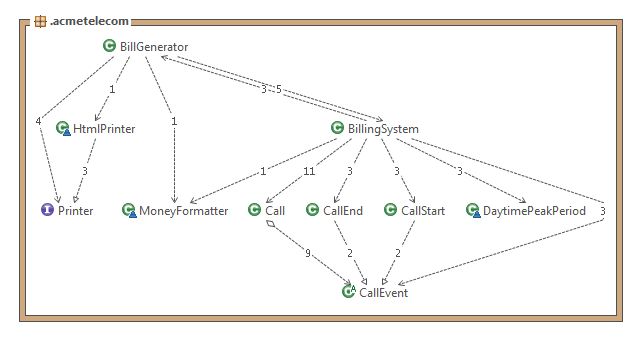
\includegraphics[scale=0.55]{images/Acme_Telecom_Structure.png}
\end{center}

\section{Testing}
Due to the importance of this system to the business, it is imperative that we ensure the correctness of the existing and new functionality. Any existing test documents or code for the system is non-existent or has been lost. Before any modifications can be made to the system we must create a comprehensive test framework. Additionally this test infrastructure will help make future changes to this system more quickly and for a lower cost.

Below we will outline our methodology for acceptance and unit testing of the existing code.

\subsection{Acceptance Testing}
It is important to test as a complete system i.e. for a given range of inputs confirm all the components interact to provide a correct result. Due to the short time-frame and to ensure correctness of the system, it was decided to involve the customer in specification of acceptance tests for the project and if possible have the customer create their own acceptance test suite. 

There are a number of approaches we may use to execute tests provided by non-technical stakeholders. These vary from parsing paragraphs of natural language to simple scripting interfaces and table based system definitions. For a project like the billing system inputs and outputs of tabular data most closely match both our programme requirements and a data format familiar to the AcmeTelecom staff in the billing department.

There are a number of open-source table based acceptance testing tools available, many of which are commonly used and have active communities. We require that the selected tool offers an interface that is simple to use and requires minimal technical knowledge enabling the customer to write parseable acceptance tests. Below we list some of the relevant testing frameworks.


\begin{itemize}
  \item Framework for Integrated Test (FIT)\\
Tests are composed of test documents, usually in HTML to define configuration, input and output parameters for a system. These documents are executed using FIT harnesses to parse the tabular data and execute it against the the system. Finally comparing expected values to the actual values in order to determine if the system meets the requirements, it output reports mirroring the input definitions. 
  \item FitNesse\\
Based on FIT, FitNesse enhances the concept through the use of a wiki environment for writing tests. This promotes increased collaboration, although we still must write fixtures test components.
  \item Concordion\\
An evolution of the FIT concept, Concordion utilises the JUnit framework for executing the tests. It offers cleaner fixture code and explicitly defined mapping through the inclusion of HTML source attributes. But these specification documents will require developer to define the mappings to fixtures.
\end{itemize}

After evaluation of the available acceptance testing tooling, we concluded that Concordion best fulfilled the requirements of the project. 

Implementation of the test fixtures required that some modifications be made to the code. These changes were necessary due to the BillingSystem being tightly coupled with BillGenerator. It was necessary to create a second constructor in the BillingSystem to pass a reference to a BillGenerator. This enabled the fixture to access the results of the call cost calculations and confirm their correctness. Changes like this were also necessary for the CustomerDatabase and TariffDatabase. 


\subsection{Unit Testing}

Due to the critical nature of the Billing System it is important to ensure regressions are not introduced during development. Before beginning feature development we implemented unit tests across much of the code, this was also helpful for the developers to become familiar with the code-base. Having this test coverage will enable the team to move more quickly and confidently in a test driven framework with the feature development.

Several unit testing frameworks are popular for Java e.g. JUnit and TestNG. These frameworks are quite similar, TestNG having the ability to execute tests in groups and begin slightly more configurable. Due to the teams experience with JUnit and the fact that Concordion integrates with it, JUnit was selected. In addition to the use of JUnit tests we also required a mechanism to ensure that the object under test is calling the correct methods on its dependency's, and to inject test data from those requests. The team members have had good previous experience using JMock and we employed its use in our testing infrastructure.

\subsubsection{Unit test implementation}
In order to test some methods it was necessary to provide mock or dummy objects for classes that we did not wish to include in the test. This mocking out of extra functionality enabled more focused and comprehensive testing.

For example in our testing of the BillingSystem.createCustomerBill(), there was an internal call to BillGenerator. We needed to ensure that BillGenerator was called, and confirm that it was called with the correct parameters but not execute any of its functionality. This type of testing resulted in us creating interfaces for many of the classes we were provided with. For the above example we created the BillGeneratorInterface for the corresponding BillGenerator.

Because the code we were provided contained a large portion of its functionality in a compiled JAR, was impossible to create interfaces for the Customer and Tariff types. In this case we created instances of these objects in the unit test and confirmed with JMock that they were being processed correctly.

During the initial unit testing we found several problems with the program’s logic:

\begin{enumerate}
	\item If there are two customers with the same telephone in the database and one of them makes a call, then they are both charged for the call (according to their price plan).
	\item If someone calls himself then he is charged for the call.
	\item If there is a CallStart event from a customer A to the customer B followed by a CallEnd event from customer A to customer C, then customer A is charged for the time between the two events.
	\item If a customer’s price plan changes, then he is charged based on the new price plan for the previous calls he has made, because all call costs are calculated after the change and not when the call has been made.
	\item If the peak and off peak hours are changed while the system is running (there are calls stored in the call log), then the call costs will be calculated based on the new peak/off peak periods.
\end{enumerate}

Using the EclEmma code coverage too for Eclipse we were able to visualise the coverage of our unit tests (screenshot attached in appendix). While code coverage is not a good measure of test comprehensiveness, it was useful for finding paths we had missed. The class we were least able to test was the Printer implementation HtmlPrinter, which outputted text to the screen using System.out.println(). We could have spend time redirecting the default system output or refactoring the class to inject an output device. We decided other areas of the system had greater priority for our efforts.

Once the team was happy with the coverage of the test for the unmodified code, the unit tests were expanded to include the new cases that would occur because of the new feature. 

\section{Feature implementation}
Given the start and end time of a call we must compute the cost depending on how many seconds are overlapping the peak period and on how many seconds are overlapping the off-peak period. To apply this change, we initially created two methods in the Call class that calculate and return the peak seconds and the off-peak seconds of the specific call. These methods are called in the BillingSystem class where we get the final cost of the call by multiplying the peak seconds returned with the specific tariff peak rate and the peak seconds with the off-peak seconds.

Having these in mind we initially converted the system milliseconds for the start and end call events into DateTime objects (using the DateTime constructor) that provides us with essential methods that are used to implement the feature.

More specifically the durationPeakSeconds() and  durationOffPeakSeconds() methods were created in the Call class. In the first method we essentially calculate the seconds of the call duration and check how many of them overlap the peak period from 7:00 to 19:00. Taking in to consideration the fact that a call duration can last more than 24 hours, more actions should be taken. One of them was to find out if and how many days existed in call duration. Next, we created a loop that iterates through the days where we create an Interval object for the peak periods for each day. Using those Interval types we compute the seconds that overlap the peak period for every day in the call. An example of the peak seconds calculation is shown below:

\begin{lstlisting}
for (int i=0;i<=daysBetween;i++){
	Interval peakHours=new Interval(peakStart.plusDays(i),peakEnd.plusDays(i));
	Interval overlapWithPeak = callInterval.overlap(peakHours);
	if (overlapWithPeak != null)
		peakSeconds+=overlapWithPeak.toDuration().getStandardSeconds();
}
\end{lstlisting}

For finding the off-peak seconds all we have to do is calculate the duration of the call in seconds and from them just subtract the peak seconds that were computed in the previous method. In the end, all that is left are the seconds overlapping the off-peak period.

Before we started analysing possible solutions for this problem we illustrated the problem by drawing a call timeline across many days, marking the intervals for OffPeak and Peak hours and then “executing” random scenarios on it. You can see an example in the following diagram

\begin{center}
	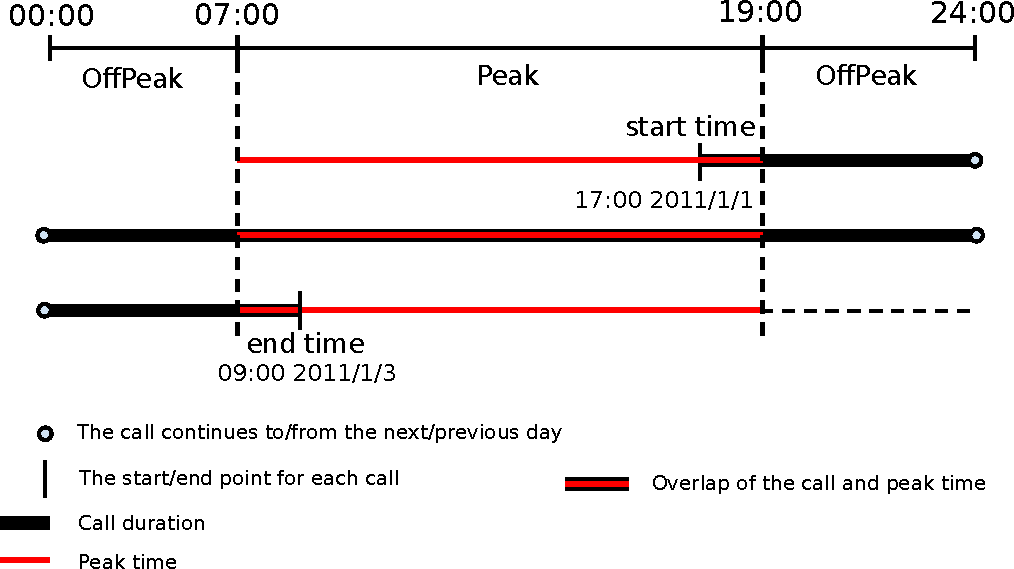
\includegraphics[scale=0.75]{images/timeline.pdf}
\end{center}

In the above diagram we simulate the case when the call starts at 17:00 in a specific day, and ends 2 days after at 05:00 and therefore lasting more than 24 hours. In this particular case we calculate the whole duration between the 2 dates in seconds which are exactly 129600 seconds (36 hours total). We then create 3 peak periods for each day and using the overlap method we calculate all the seconds from the call duration that overlap the peak periods. After computing the peak seconds we also compute the off-peak seconds by subtracting the peak seconds from the whole call duration.
\section{Additional Changes}

\subsection{DSL like logging interface}
During development it was found that the callInitiated() and callComplete() methods in the Billing System were prone to error. It was easy for a developer to initialise the call in the wrong order i.e. callInitiated(callee, caller), creating major billing issues.

To combat this we redesigned the call logging interface. This new interface relies on the autocompletion features of modern IDE's by returning the 'this' value cast to a particular interface. With this we used domain specific language to create interface.
\begin{lstlisting}
	billingSystem.startCall().from(caller).to(callee);
\end{lstlisting}
To implement this feature a CallLogInterface interface was created, and the BillingSystem implemented this 'role'. The startCall() method creates a new object which builds the data necessary to log an entry, and calls the callInitiated() method of BillingSystem.

To direct new users to this interface and maintain backwards compatibility we added Javadoc and the @deprecated annotation to the callInitiated()  and callComplete() methods. It would have been possible to go even further an create mini-types for the call data, but we felt this would have been too great of a change for this release.

\subsection{Externalise configuration parameters}
In order for the values for the peak and off-peak times to be easily modified these where externalised to a properties file. An external properties file was created to store keys for peak\_start\_time and off-peak\_start\_time. These times can be changed in the future simply by editing the properties file.

The file is loaded through a loadConfigurationProperties() method that is called in the constructor of the BillingSystem class. 

\begin{lstlisting}
props.load(new FileInputStream("billing_system.properties"));
if(props.containsKey(PEAK_RATE_START_TIME))
	peak_rate_start = props.getProperty(PEAK_RATE_START_TIME);
if(props.containsKey(OFF_PEAK_RATE_START_TIME))
     	off_peak_rate_start = props.getProperty(OFF_PEAK_RATE_START_TIME);
if (off_peak_rate_start == null || peak_rate_start == null)
	throw new Exception("Configuration error!");	
\end{lstlisting}

Moving these and future values to a configuration file will enable the business to be more responsive and cost effective.

\subsection{More comprehensive time framework}
Refactoring the code to implement the changes was difficult using the standard JDK Date library. Because of that, other libraries were researched for implementing dates and times in Java more effectively. We found some external libraries built especially to solve problems with the standard classes like Date4j and JodaTime. After some evaluations of the two libraries we decided that the JodaTime Project that provides a quality replacement for the internal Date and Time classes. It supports all the methods that already exist in the JDK Date but provides even more features and useful types. Additionally, there are conversion methods between the JDK class Date and the JodaTime DateTime type. JodaTime has been designed to fix numerous bugs that exist in the JDK classes date and time and also to improve performance. A great advantage of using the JodaTime is that it enables much easier testing with various methods. 

An example of using JodaTime DateTime:
\begin{lstlisting}
	DateTime dateTime = DateTime.parse(date, DateTimeFormat.forPattern("dd/MM/yy HH:mm:ss"));
	billingSystem.startCall().atTime(dateTime.getMillis()).from(caller).to(callee);
	billingSystem.endCall().atTime(dateTime.plusSeconds(durationSeconds).getMillis()).from(caller).to(callee);
\end{lstlisting}

Lastly, we made sure that this library is safe to be used in the system in terms of maturity. Under active development since 2002 (last release was in June this year) and it continues to receive new features and bug-fixes. Some other helpful classes and methods included in the JodaTime project are described next.

\subsubsection{Duration between two dates}
Using the Duration class included in the JodaTime project we can easially calculate the duration between two DateTime instances. Included in the Duration class, are various methods, that return the duration of the two dates in days, hours, seconds and milliseconds. An example of returning the seconds between two dates is showed below:
\begin{lstlisting}
	Duration callDuration=new Duration(dtStartCall, dtEndCall);
	int durationInSeconds=callDuration.getStandardSeconds();
\end{lstlisting}

\subsubsection{Integration of JodaTime}
Some modifications to the system had to be done in order for the standard dates to be replaced by the DateTime types. A number of them were made to the Call.java class where were Dates for the startTime and endTime of the call were being returned. Another necessary modification applied was in the DaytimePeakPeriod in order for the offPeak method to accept DateTime argument instead of the standard JDK Date type.
\begin{lstlisting}
public boolean offPeak(DateTime time) {     
	int hour = time.getHourOfDay();
	return hour < peak_rate_start || hour >= off_peak_rate_start;
}
\end{lstlisting}
\newpage
\section{Appendix}

\subsection{Source code}
During development the project was managed using GIT. This reduced the time required for integration of features and the ease at which all the team members were kept up to date.\\
The project is available at:
\begin{lstlisting}
https://github.com/johnflan/Advanced-Topics-in-Software-Engineering---Coursework-2
\end{lstlisting}

\subsection{Unit test coverage}
\begin{center}
	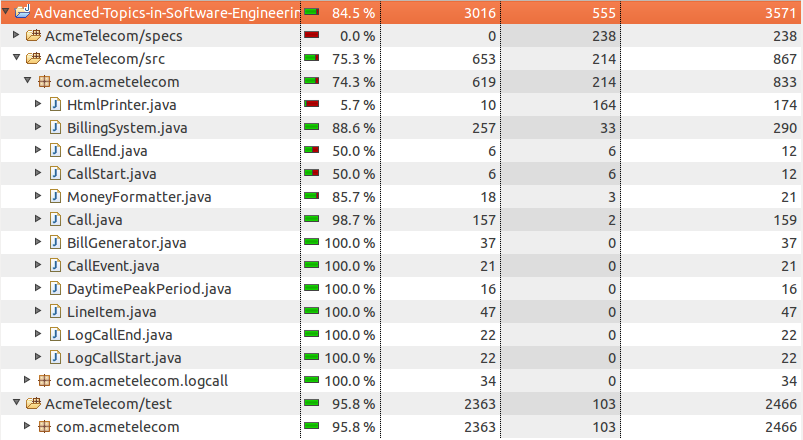
\includegraphics[scale=0.55]{images/emma_code_coverage_.png}
\end{center}

\subsection{Initial and Final dependency diagrams}

\begin{center}
	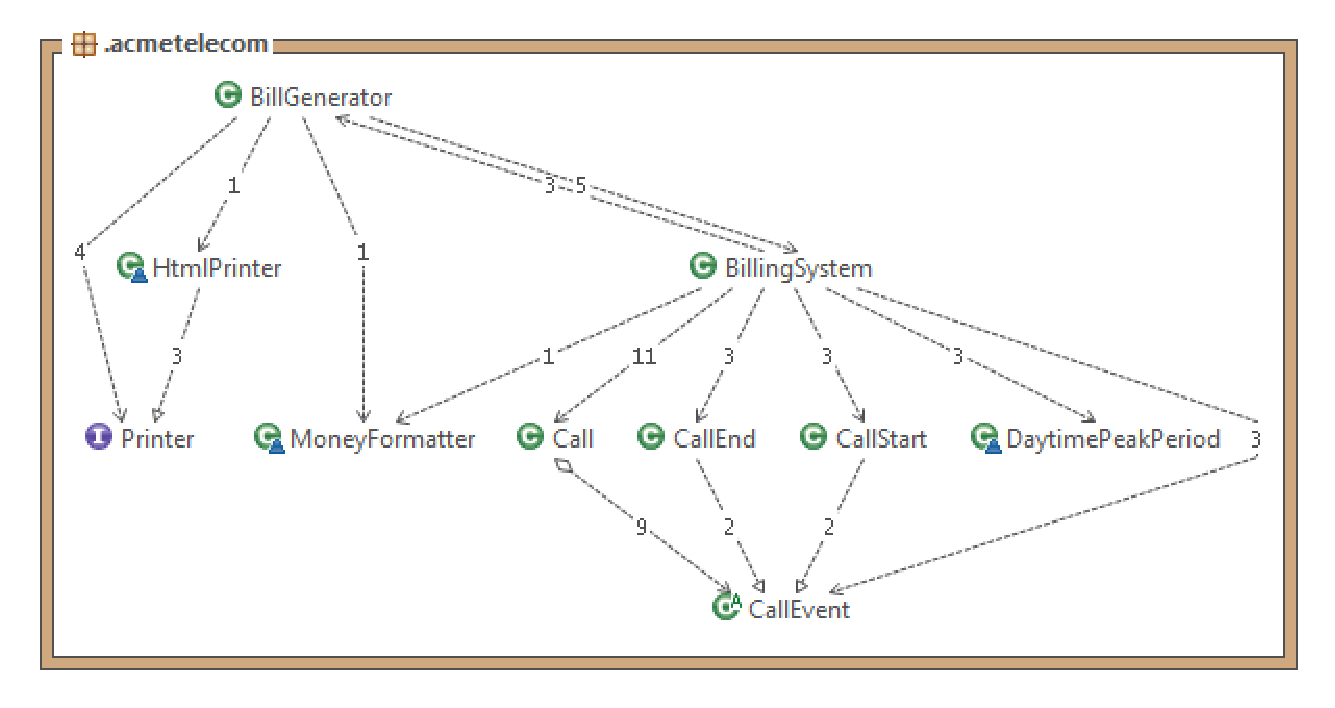
\includegraphics[scale=0.7]{images/Acme_Telecom_Structure.pdf}
Initial dependency structure
\end{center}

\begin{center}
	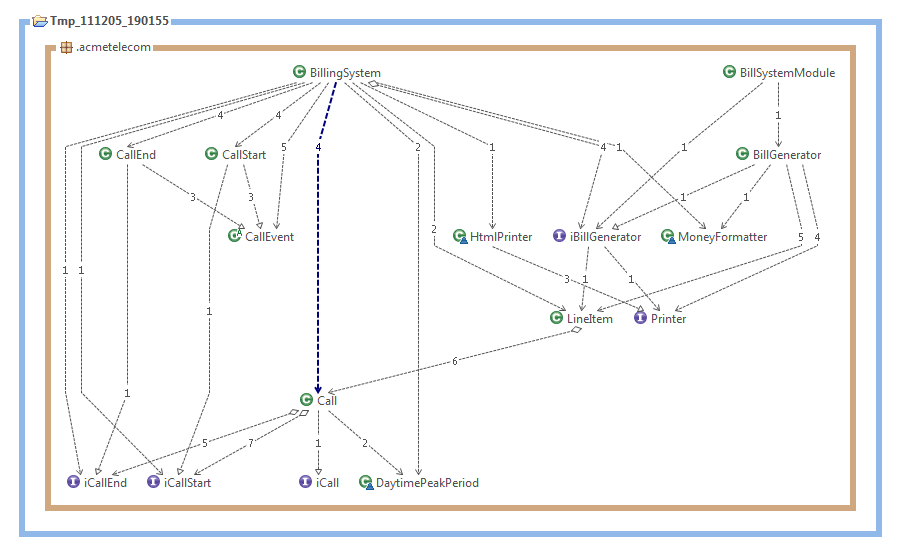
\includegraphics[scale=0.45]{images/AcmeTelecom_Software_Structure_After_Refactoring.png}\\
Structure after feature development
\end{center}

\subsection{Initial Acceptance Test}
\begin{center}
	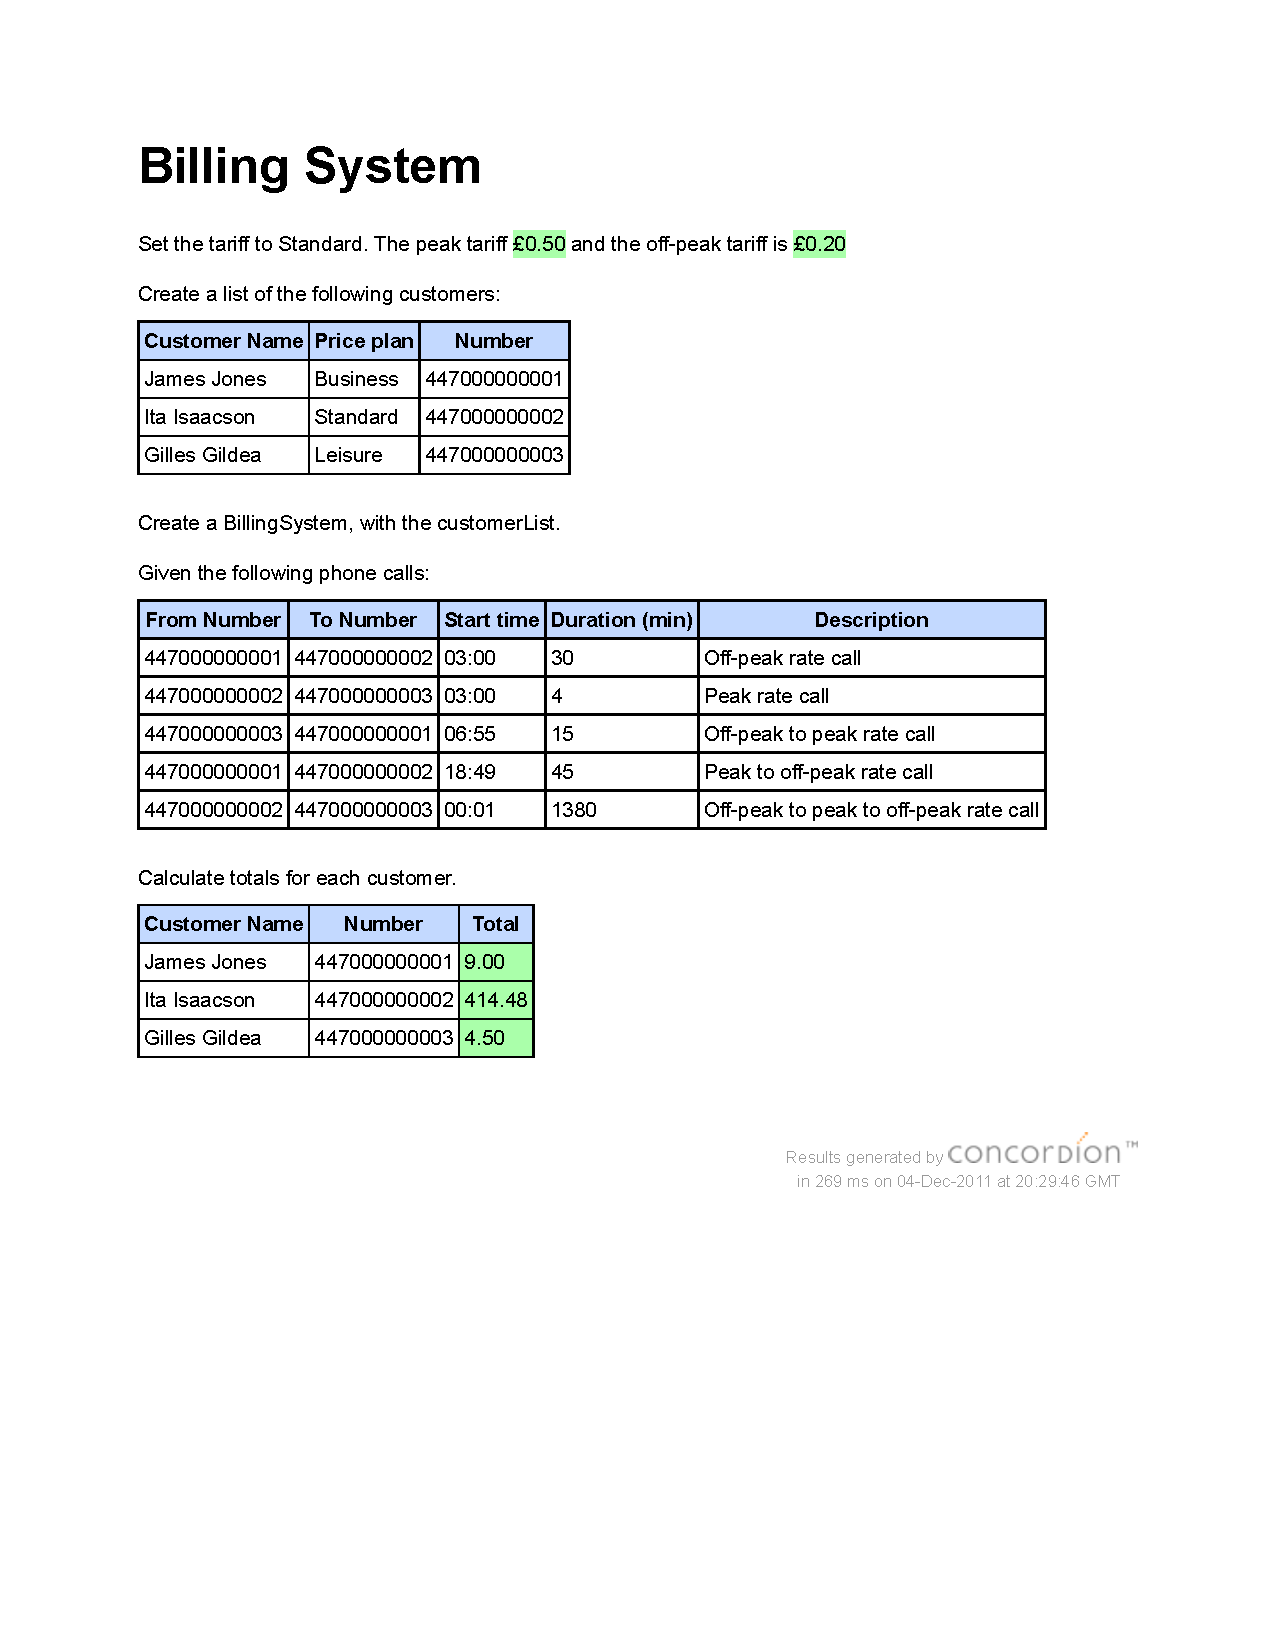
\includegraphics[scale=0.7]{images/InitialAcceptanceTest.pdf}
\end{center}
\end{document}
